% %This is a very basic article template.
% %There is just one section and two subsections.
\documentclass[a4paper,12pt]{article}
\usepackage{cite}
\usepackage{graphicx}
\usepackage{float}

\begin{document}


\section{Classifying EUNIS Habitats Using Ontologies and Data Mining Methods}

\section{Introduction - Context and Background}
Recognizing that human-caused habitat destruction plays a dominant role in
biodiversity loss, the European Union has implemented an environmental
conservation framework to halt biodiversity law in accordance with the
Convention on Biological Diversity (CBD, 2005). An integral part of this
framework is the EU Habitats Directive (Council Directive) 92/43/EEC [1992],
which established the Natura 2000 network of habitats. The law requires
conservation and monitoring of designated habitats by member states and for a
report to be submitted every six years. 

Earth Observation data can be combined with  local knowledge are

Yet as Lucas et. al (2015) point out there are no standards for classifying
habitats with Earth Observation (EO) data that can be applied to all sites. 

Due to differing standards and approaches of the various nature conservation
agencies in collecting and disseminating information, data comparison is
difficult. Different data types and data sources increase the difficulty in
comparing data from one site to another. Furthermoe, habitat monitoring can
be labor intensive and subjective.

Luckily, EO data could help reduce the burden of environmental monitoring and
also provide information on conservation status.

An automated system that can classify Natura 2000 habitats using EO
data and an existing biotope map as inputs would greatly increase monitoring
comparability and accuracy. 

We propose an automated system using 
EU-wide biotope classification schema called European Union Nature Information
System (EUNIS), data mining algorithms for training on biotope data and
ontologies for hierarchical reasoning and information management.

\section{State of Research and Research Question}
Remote sensing has a rich history in environmental conservation, meteorology,
climate science and other fields. Due to this history remote sensing experts
have become very good at analyzing remote sensing data. Yet, remote sensing
image analysis implicitly incorporates the expertise and knowledge of the
individual performing the analysis and reduces objectivity. This can be divided
into remote sensing knowledge (spectral signature, remote sensing index, etc.)
and field knowledge (feature properties, spatial relations, etc)
\cite{Andres2013a}. This knowledge is often neither completely nor explicitily
defined but influences the classification. Thus, two experts can interpret the
same image differently due to their unique conceptualizations and experiences.
Further complicating matters, the classification chain is not documented and
controlled, reducing comparability and hindering attempts to reproduce the
results\cite{Arvor2013}. Therefore (semi) automatic methods for remote sensing
classifications that produce accurate and reproducible results are desired.
A (semi) automatic system would also reduce the time needed to analyze large
remote sensing datasets. Many approaches have been used to create an accurate
(semi) automatic classification tool using statistics and different algorithms
from machine learning and data mining. Unfortunately most of these approaches
rely on experts to produce rule-sets or manually select training points. The
former relies on \emph{a priori} knowledge while the latter can be
time-consuming.
Neither are observation-based. There are many different (semi) automatic methods
for feature selection. A brief overview explaining the most common methods is
described below.

\subsection{Background - Remote Sensing and Ontologies}

\subsection{Feature selection}
%% focus on ML?

There are many different classification approaches with varying degrees of
complexity and requiring different levels of user input. One commonly used
classification approach, the maximum likelihood classification (MLC) approach,
among the most popular, has been used to study land use change in China
\cite{Ding2007}, analyze forest cover in Haiti \cite{Churches2014} and land
cover and land-use change in Egypt \cite{Shalaby2007}. Recent research suggests
support vector machines (SVMs) when compared to decision trees (DTs), a neural
network classifier and the MLC, produces better results \cite{Huang2002}. One
such DT is the ``Random Forest'' algorithm which has been shown to be better
than Adaboost \cite{Chan2008} and performed well when applied to the Cape Cod
National Seashore for coastal dune and salt marsh classification
\cite{Timm2012}.
% need more?
Yet these algorithms are more suited for pixel-based image analysis and do not
allow for automatic derivation of thresholds for classes.
% % more examples of data mining/machine learning?

\subsection{Selection of Algorithm}
The Separability and Thresholds
(SEaTH) \cite{Nussbaum2006} algorithm to automatically derive features important
for classification from the data.
\subsection{Empirically derived feature selection and threshold delineation -
SEaTH} The Separability and Thresholds (SEaTH) algorithm \cite{Nussbaum2006}
statistically identifies characteristic features and their thresholds. It has
been used on remote sensing data for land cover classification \cite{Gao2011}
and nuclear installation classification \cite{Nussbaum2006}.
Using training data, the algorithm determines the separability of the object
classes and then calculates the thresholds for which the maximum separability
can be achieved using the given features. One benefit of the algorithm is that
one does not need many training objects.
In the Nussbaum, Niemeyer and Canty (2006) paper, for example, the authors
suggest using only very characteristic features for training and only used
around 10 samples per class\cite{Nussbaum2006}. The authors also state that
usually two features per class is enough to produce accurate results. Combining
this algorithm with an ontology would produces traceable results that are easy
to understand. This approach would also help fill the observation-based ontology
research gap as first described by Janowicz (2012) \cite{Janowicz2012}.
\subsection{Comparison with Extra Trees Classifier}
We compare the results of the SEaTH tool with the Extra Trees classifier
implemented in scikit-learn\cite{scikit-learn}.

\subsection{Semantic-based image interpretation}
Different fields (medical imaging, security, etc.) have used ontologies for
improving image retrieval and object detection. Only recently have ontologies
been adopted in remote sensing research. An ontology, defined as ``an explicit
specification of a conceptualization'' \cite{gruber1993} could help bridge the
semantic gap and allow for better data interoperability, workflow management and
automatic image interpretation \cite{Arvor2013} \cite{Andres2013a}. The term
``semantic gap'' refers to the difference between the higher-level descriptions
by experts and what can be extracted from the visual data. Remote sensing and
field expert knowledge can be digitized in ontologies, thus allowing for a
hierarchy of concepts for improved automatic image annotation and retrieval
using concepts from both fields to produce more accurate results
\cite{Srikanth:2005:EOA:1076034.1076128}. Janowicz \cite{Janowicz2012}
advocates for more observation-driven ontologies and for including machine
learning, geostatistics and data mining to construct ontological primitives.
Research on using observation-based ontologies for classifications is still
lacking. There are initiatives to use ontologies in biodiversity research. Below
are some examples.
\subsection{Ontologies in remote sensing research}
One such research project is the EU-funded ``Biodiversity Multi-Source
Monitoring System:
From Space To Species'' (BIO\_SOS) which seeks to develop tools to monitor and
map protected areas in the EU and uses ontologies modeled on the Land Cover
Classification System (LCCS) and the General Habitat Category (GHC) to achieve
this goal \cite{Arvor2013}. Using the taxonomy of the different classification
systems allows expert knowledge to be included in the process.
Further work as part of the project includes creation of a standardized
framework for habitat monitoring and mapping called the Earth Observation Data
for Habitat Montioring (EOD-HAM) system \cite{Lucas2015}. The system harnesses
knowledge from both remote sensing and ecology to classify Natura 2000 sites
using a hierarchical classification system. The EOD-HAM system uses both
pixel-based analysis and OBIA for greater classification accuracy but still
relies on a rule-base created by an expert or the user. Other research includes
a semi-automatic semantic classification approach for urban building types using
a three-layered architecture was developed by di Sciascio et al. which showed
promising results \cite{diSciascio2013}. Belgiu et al. \cite{Belgiu2014} used
Airborne Laser Scanning (ALS) data and empirically determined thresholds using
the Random Forest (RF) classifier to perform an ontology-based classification of
building types. Forestier et al. \cite{Forestier2012470} used an ontology to
classify pre-segmented regions using a knowledge-base. Sheeren et al.
\cite{Sheeren2006ML} developed a method to automatically acquire classification
rules using a newly developed genetic programming algorithm called 'ProgGen'.
Sheeren et al. also used the data mining algorithm C4.5 for automatic rule
generation with satisfactory results. Nieland et al. \cite{Nieland2015}
demonstrated the potential for ontological inference and hierarchical
matchmaking as a way to improve spatial data interoperability. An automated
image analysis and classification process that could be applied to the whole
Natura 2000 network would be ideal and allow for comparison between habitats.
Such an automated tool could combine the benefits of object-based image analysis
(OBIA) with linguistic terms for a traceable and reproducible classification
system. When an ontology is available, scientists can follow how the classes
were developed and become aware of possible incompatibilities before combining
datasets \cite{Janowicz2012}.

\subsection{Research Question}
\begin{itemize}
  \item Does the proposed methodology produce accurate/valid results?
  \item Can the method be applied to other classes with similar accuracy?
\end{itemize}
\section{Method}
\subsection{Input Data into Workflow}
After joining EUNIS characteristics to the RLP biotope map, the map was 
spatially joined with the pre-segmented remote sensing data. Defiens eCognition
software was used for the segmentation and was performed by RLP AgroScience. 
The remote sensing data already had zonal statistics computed for all of the
polygons.
\begin{itemize}
  \item min, max, mean, median, sum and stddev of:
  \begin{itemize}
    \item aspect, caar,
	\item coin
	\item difi
	\item diri
	\item diah
	\item flac
	\item mrrt
	\item mrvb
	\item prcu
	\item slop
	\item swi
	\item toin
  \end{itemize}with  sum and stddev of 
\end{itemize}

%% ROC? Recall Percision? Evaluation of quality?

\subsection{Environmental Data}

9 Segmentation Classes from ecognition:
'BodenOffen', 'BodenVegKarg', BodenVegMittel', 'BodenVegSchwach',
'BodenVegStark', 'NoVeg', NoVegHoch', 'Plantagen', 'Veg'


\subsection{Study Area and Data}
The study area is located in the southeastern part of the Trier-Saarbug district
in the federal state of Rhineland-Palatinate, Germany. At approximately
200km$^{2}$, Luxembourg borders the district to the west and the federal state of Saarland to the South.
\begin{figure}
	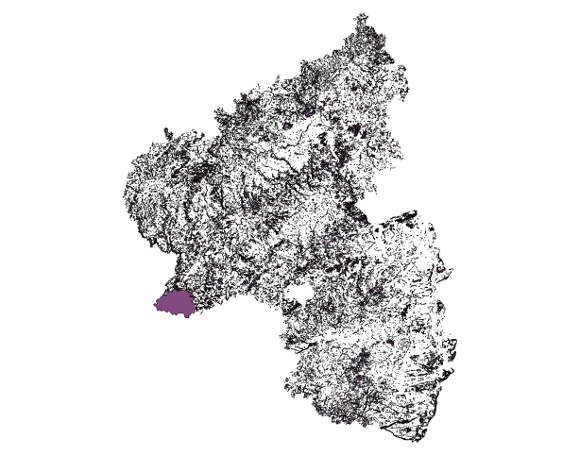
\includegraphics[width=\textwidth]{diagrams/study_area_small.png}
\end{figure}

\section{Results}
\subsection{Feature importance}
The single dimension (SEaTH) and multi-dimensional classification
algorithms chose very different features as important. While SEaTH performs
better when trained on a few objects displaying characteristic
features\cite{Nussbaum2006}, the extra trees classifier and other ensemble
algorithms generally are trained on a larger portion of the data. To compare
performance more appropriately, we train SEaTH on a small dataset and the same
dataset used for the extra trees classifier.


We use WEKA and a cross-validation of 10 to train a J48 algorithm on the data.

SEaTH classification accuracy depended on the the number of features used to cS


\section{Discussion}
SEaTH shows much better separability when one chooses larger objects and fewer
from each object. Training SEaTH on few carefully selected objects being ideal
representations of the class further increases the separability. Using two sets
of rules produced from different sized training data produced quite different
results when tested on the same dataset. 
%% are some ogc_fids in training in testing data? 
\section{Conclusion}

\end{document}
